\section{Ejercicio 1}
		Computaciones para el programa
		\begin{verbatim}
		J(2,3,0)
		S(1)
		S(3)
		J(1,1,1)
		\end{verbatim}
  		\subsection{Computación para la entrada $R1=0, R2=0$}
		\begin{equation*}\begin{gathered}
		(1, <R1=0, R2=0, R3=0>) \sim (0, <R1=0, R2=0, R3=0>)
		\end{gathered}\end{equation*}
		\begin{figure}[H]
  			\centering
  			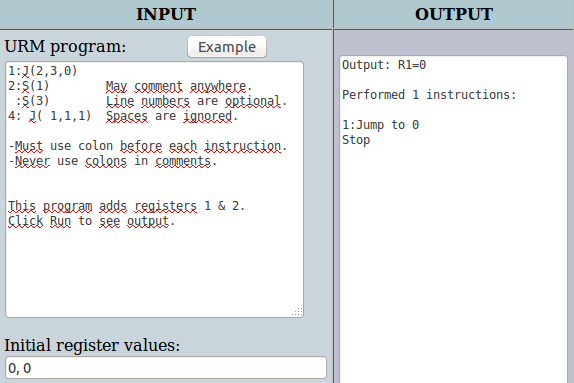
\includegraphics[scale=0.5]{images/100.png}
  		\end{figure}
		\subsection{Computación para la entrada $R1=1, R2=1$}
		\begin{equation*}\begin{gathered}
		(1, <R1=1, R2=1, R3=0>) \sim (2, <R1=1, R2=1, R3=0>) \sim (3, <R1=2, R2=1, R3=0>) \sim\\
		(4, <R1=2, R2=1, R3=1>) \sim (1, <R1=2, R2=1, R3=1>) \sim (0, <R1=2, R2=1, R3=1>)
		\end{gathered}\end{equation*}
		\begin{figure}[H]
  			\centering
  			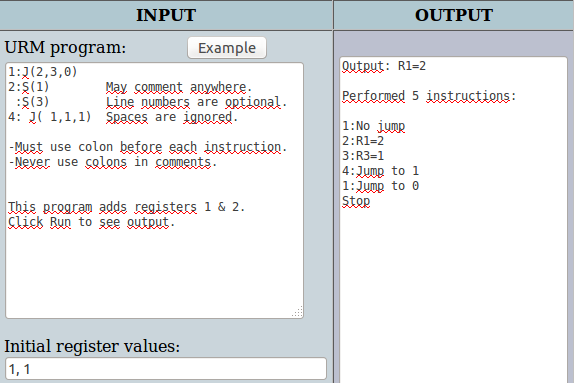
\includegraphics[scale=0.5]{images/111.png}
  		\end{figure}
		\subsection{Computación para la entrada $R1=1, R2=2$}
		\begin{equation*}\begin{gathered}
		(1, <R1=1, R2=2, R3=0>) \sim (2, <R1=1, R2=2, R3=0>) \sim (3, <R1=2, R2=2, R3=0>) \sim\\
		(4, <R1=2, R2=2, R3=1>) \sim (1, <R1=2, R2=2, R3=1>) \sim (2, <R1=2, R2=2, R3=1>) \sim\\
		(3, <R1=3, R2=2, R3=1>) \sim (4, <R1=3, R2=2, R3=2>) \sim (1, <R1=3, R2=2, R3=2>) \sim\\
		(0, <R1=3, R2=2, R3=2>)
		\end{gathered}\end{equation*}
		\begin{figure}[H]
  			\centering
  			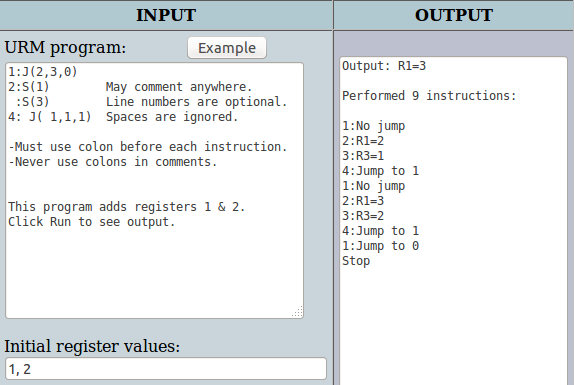
\includegraphics[scale=0.5]{images/112.png}
  		\end{figure}
		\subsection{Computación para la entrada $R1=2, R2=1$}
		\begin{equation*}\begin{gathered}
		(1, <R1=2, R2=1, R3=0>) \sim (2, <R1=2, R2=1, R3=0>) \sim (3, <R1=3, R2=1, R3=0>) \sim\\
		(4, <R1=3, R2=1, R3=1>) \sim (1, <R1=3, R2=1, R3=1>) \sim (0, <R1=3, R2=1, R3=1>)
		\end{gathered}\end{equation*}
		\begin{figure}[H]
  			\centering
  			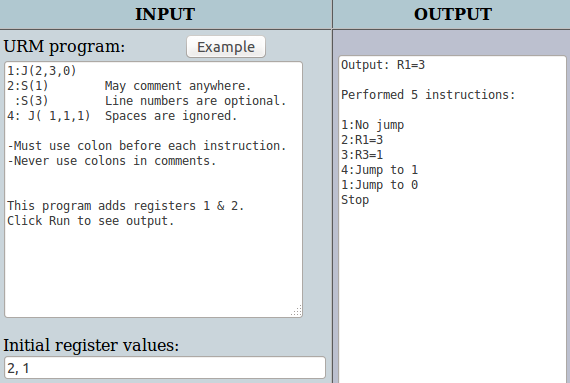
\includegraphics[scale=0.5]{images/121.png}
  		\end{figure}
